%%%%%%%%%%%%%%%%%%%%%%%%%%%%%%%%%%%%%%%%%
% Beamer Presentation
% LaTeX Template
% Version 1.0 (10/11/12)
%
% This template has been downloaded from:
% http://www.LaTeXTemplates.com
%
% License:
% CC BY-NC-SA 3.0 (http://creativecommons.org/licenses/by-nc-sa/3.0/)
%
%%%%%%%%%%%%%%%%%%%%%%%%%%%%%%%%%%%%%%%%%

%----------------------------------------------------------------------------------------
% PACKAGES AND THEMES
%----------------------------------------------------------------------------------------

\documentclass{beamer}

\mode<presentation> {

% The Beamer class comes with a number of default slide themes
% which change the colors and layouts of slides. Below this is a list
% of all the themes, uncomment each in turn to see what they look like.

%\usetheme{default}
%\usetheme{AnnArbor}
%\usetheme{Antibes}
%\usetheme{Bergen}
%\usetheme{Berkeley}
%\usetheme{Berlin}
%\usetheme{Boadilla}
%\usetheme{CambridgeUS}
%\usetheme{Copenhagen}
%\usetheme{Darmstadt}
%\usetheme{Dresden}
%\usetheme{Frankfurt}
%\usetheme{Goettingen}
%\usetheme{Hannover}
%\usetheme{Ilmenau}
%\usetheme{JuanLesPins}
%\usetheme{Luebeck}
\usetheme{Madrid}
%\usetheme{Malmoe}
%\usetheme{Marburg}
%\usetheme{Montpellier}
%\usetheme{PaloAlto}
%\usetheme{Pittsburgh}
%\usetheme{Rochester}
%\usetheme{Singapore}
%\usetheme{Szeged}
%\usetheme{Warsaw}

% As well as themes, the Beamer class has a number of color themes
% for any slide theme. Uncomment each of these in turn to see how it
% changes the colors of your current slide theme.

%\usecolortheme{albatross}
%\usecolortheme{beaver}
%\usecolortheme{beetle}
%\usecolortheme{crane}
%\usecolortheme{dolphin}
%\usecolortheme{dove}
%\usecolortheme{fly}
%\usecolortheme{lily}
%\usecolortheme{orchid}
%\usecolortheme{rose}
%\usecolortheme{seagull}
%\usecolortheme{seahorse}
%\usecolortheme{whale}
%\usecolortheme{wolverine}

%\setbeamertemplate{footline} % To remove the footer line in all slides uncomment this line
%\setbeamertemplate{footline}[page number] % To replace the footer line in all slides with a simple slide count uncomment this line

%\setbeamertemplate{navigation symbols}{} % To remove the navigation symbols from the bottom of all slides uncomment this line
}
\usepackage{amsthm,amsmath,amssymb,upgreek,marvosym,mathtools}
\usepackage{graphicx}
\usepackage{multirow,bigdelim}
\graphicspath{ {./pics/} }

\usepackage{booktabs} % Allows the use of \toprule, \midrule and \bottomrule in tables
\usepackage{xcolor}
\usepackage{fancyvrb}
\usepackage{float}
\usepackage{pgffor}% http://ctan.org/pkg/pgffor
\usepackage{pdfpages}
\usepackage{pifont}% http://ctan.org/pkg/pifont
\usepackage{subfig}
%\newtheorem{lemma}{Lemma}
\newtheorem{reduction}{Reduction}
\newtheorem{proposition}{Proposition}
\newtheorem{claim}{Claim}
\newtheorem{scolium}{Scolium}   %% And a not so common one.
%\newtheorem{definition}{Definition}
\newtheorem{construction}{Construction}
\usepackage[export]{adjustbox}
\usepackage{appendixnumberbeamer}

\usepackage{tkz-graph}
\usepackage{arydshln}
\usepackage{comment}
\setbeamertemplate{enumerate items}[default]
\usetikzlibrary{automata, positioning,arrows,shapes,decorations.pathmorphing}
\newcommand{\distras}[1]{%
  \savebox{\mybox}{\hbox{\kern3pt$\scriptstyle#1$\kern3pt}}%
  \savebox{\mysim}{\hbox{$\sim$}}%
  \mathbin{\overset{#1}{\kern\z@\resizebox{\wd\mybox}{\ht\mysim}{$\sim$}}}%
}
 \tikzset{
node distance=3cm, % specifies the minimum distance between two nodes. Change if necessary.
every state/.style={thick, fill=gray!10}, % sets the properties for each ’state’ node
initial text=$ $, % sets the text that appears on the start arrow
}

\newcommand{\db}{$\mathbf{db}$}
\newcommand{\sjfq}{\texttt{sjfCQA}}
\newcommand{\bcq}{\texttt{bcq}}
\newcommand{\prob}[1]{\textsc{certainty}($#1$)}
\newcommand{\fo}{$\mathbf{FO}$}
\newcommand{\p}{$\mathbf{P}$}
\newcommand{\lspace}{$\mathbf{L}$}
\newcommand{\coNP}{$\mathbf{coNP}$}
\newcommand{\und}[1]{\underline{#1}}
\newcommand{\nl}{$\mathbf{NL}$}
\newcommand{\sel}[1]{\sigma_{\text{#1}}}

\title[Accelerating Joins with Filters]{Accelerating Joins with Filters} % The short title appears at the bottom of every slide, the full title is only on the title page

\author{Nicholas Corrado \and Xiating Ouyang} % Your name
\institute[] % Your institution as it will appear on the bottom of every slide, may be shorthand to save space
{
University of Wisconsin-Madison \\ % Your institution for the title page
\medskip
\textit{} % Your email address
}
\date{} % Date, can be changed to a custom date




\begin{document}

\begin{frame}
\titlepage % Print the title page as the first slide
\end{frame}


\begin{frame}
\frametitle{Star Schema}

\begin{figure}
    \centering
    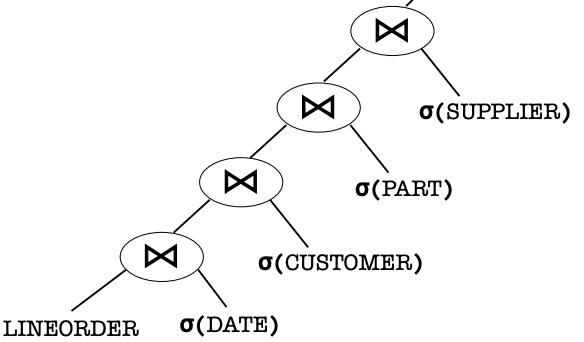
\includegraphics[height=0.5\textheight,keepaspectratio]{join-tree}
\end{figure}

\begin{itemize}
  \item If the query optimizer chooses a poor join order, intermediate join results may be unnecessarily large.
  \item Solution: try to filter out extraneous tuples before performing joins
\end{itemize}
\end{frame}

% lip slides here



\foreach \n in {1,...,25} {%
  \begin{frame}[noframenumbering]
  \frametitle{Lookahead Information Passing (LIP)}
  \begin{figure}
    \centering
    \includegraphics[page={\n},height=0.7\textheight,keepaspectratio]{lip-animation}
    \end{figure}
  \end{frame}
}


\begin{frame}[noframenumbering]
  \frametitle{Lookahead Information Passing (LIP)}
  \begin{figure}
    \centering
    \includegraphics[page={26},height=0.7\textheight,keepaspectratio]{lip-animation}
  \end{figure}
  
\end{frame}
% lip slides above

\begin{frame}
  \frametitle{LIP-$k$}

  \begin{itemize}
    \item LIP uses statistics from all previous batches to compute $\sigma$
    \begin{itemize}
        \item Slow response to local changes in key distributions in fact table
        \item e.g.\ $(11/28/2019, \text{Turkey})$
    \end{itemize}
    \item \textbf{LIP-k}: Only use the previous $k$ batches to compute $\sigma$
  \end{itemize}

\end{frame}


\begin{frame}
  \frametitle{Implementation and benchmarking}
  \begin{figure}
    \centering
    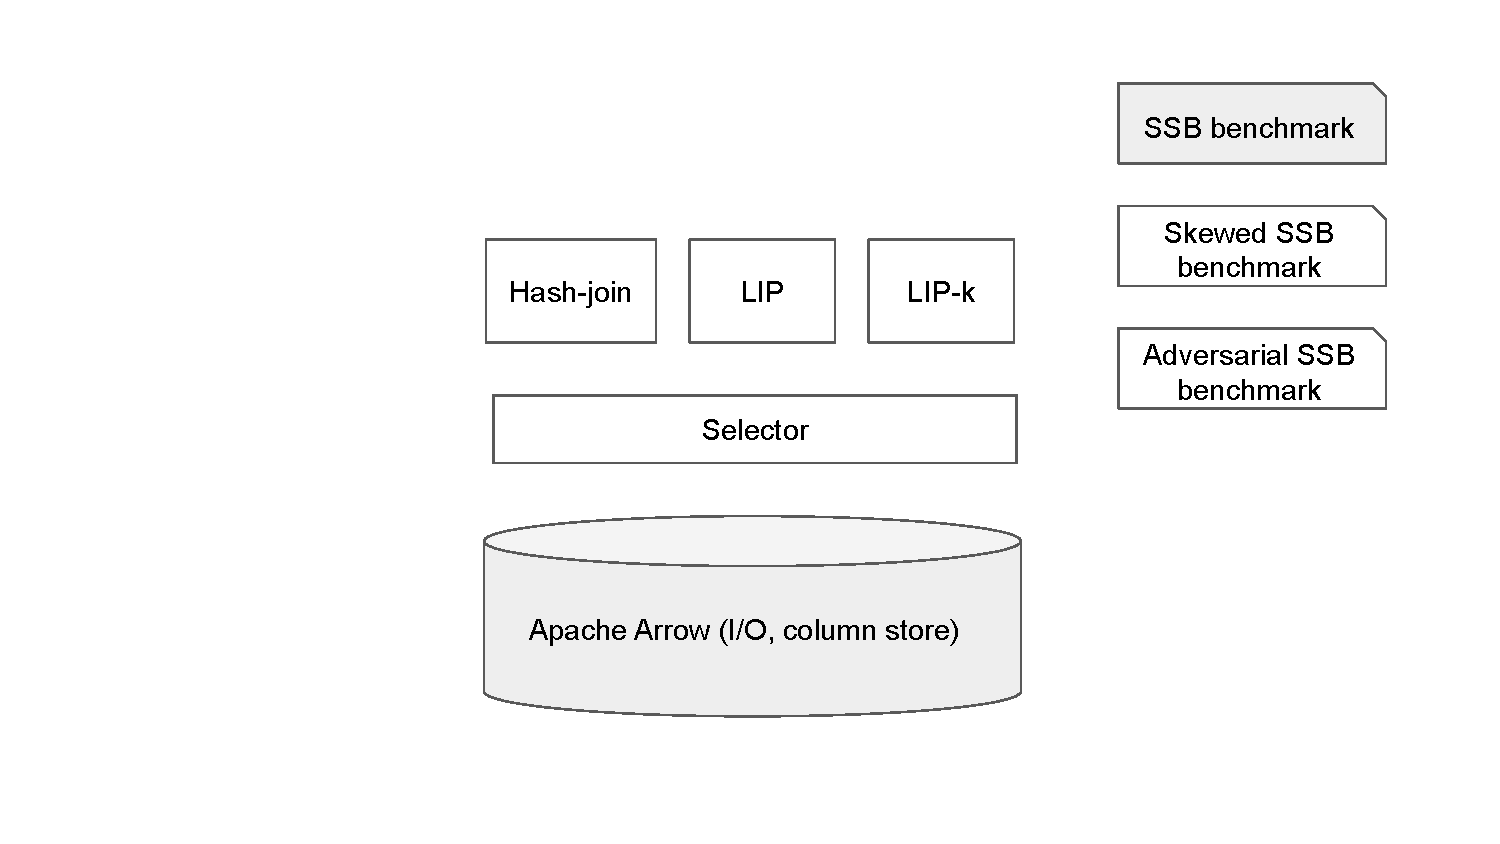
\includegraphics[height=0.7\textheight,keepaspectratio]{implementation}
  \end{figure}
\end{frame}


\begin{frame}
  \frametitle{An Example Experiment}
  \begin{itemize}
    \item Select where \texttt{Credit Score }$\geq 700$
  \end{itemize}
  \vspace{-0.5cm}
  \begin{columns}
    \begin{column}{0.25\textwidth}
        \small
        \begin{tabular}{c c}
         \texttt{Credit Score} \\
         \hline
         720 & \rdelim \} {4}{3mm}[50 batches] \\
         750 & \\
         720 & \\
         $\dots$ \\
         \hline
         400 & \rdelim \} {4}{3mm}[50 batches]\\
         400 & \\
         400 & \\
         $\dots$ \\
         \hline
         770 & \rdelim \} {4}{3mm}[50 batches]\\
         810 & \\
         800 & \\
         $\dots$  
        \end{tabular}

    \end{column}
    \begin{column}{0.7\textwidth}
    \begin{figure}
    \hspace*{2cm}
      \centering
      \begin{overprint}
            \onslide<2>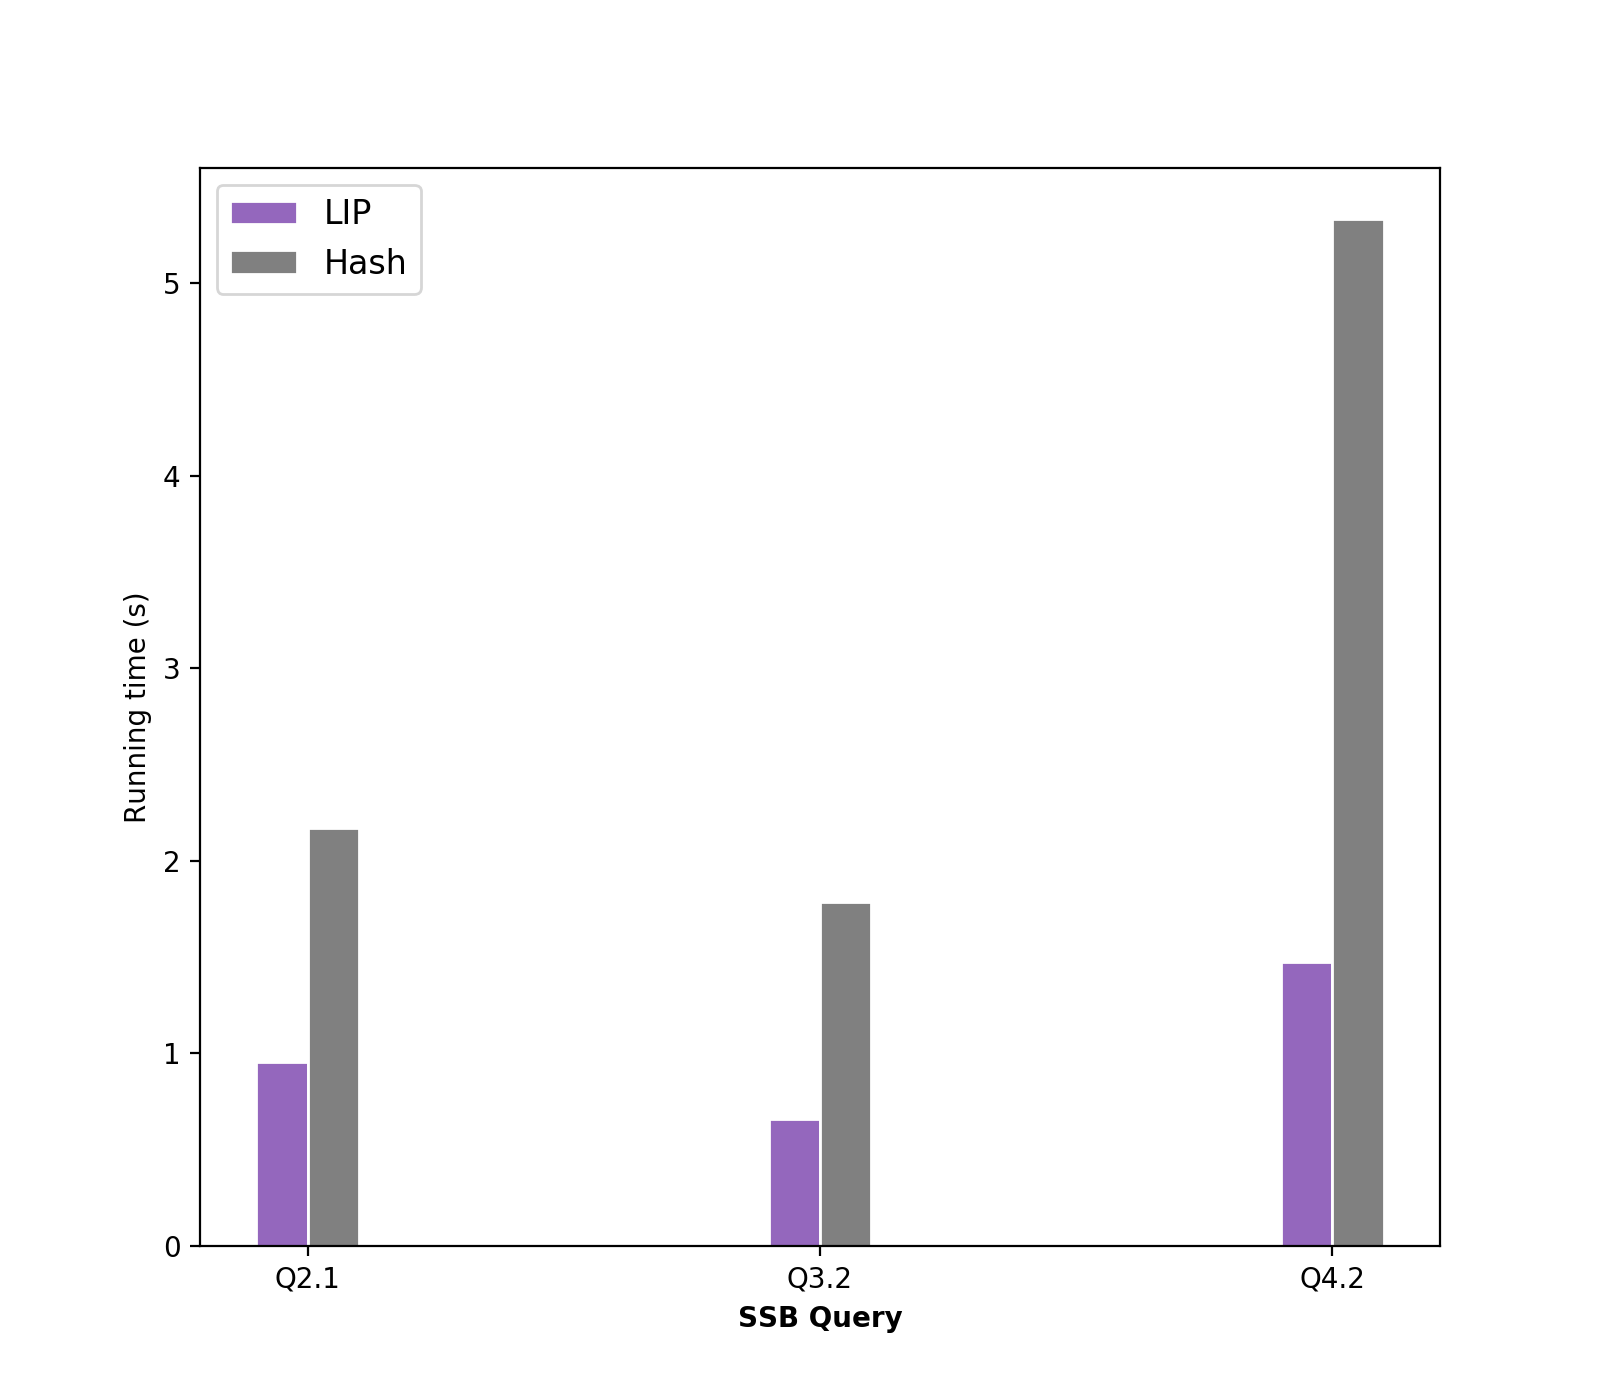
\includegraphics[width=0.8\textwidth,keepaspectratio]{time-graph-hash}
            \onslide<3->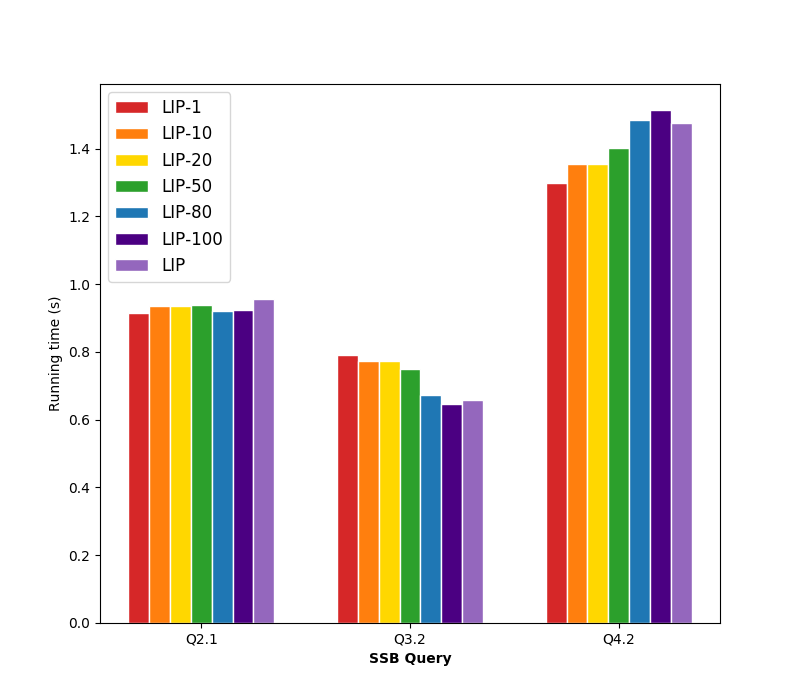
\includegraphics[width=0.8\textwidth,keepaspectratio]{time-graph-no-hash}
      \end{overprint}
    \end{figure}
    \end{column}
  \end{columns}


  \begin{itemize}
      \visible<4->{\item LIP-$k$ performs better than LIP on some queries...}
      \visible<5->{\item ...but LIP performs better on others}
  \end{itemize}
\end{frame}


\begin{frame}
\frametitle{LIP is solving an online problem}
\begin{itemize}
  \visible<1->{\item Given any tuple $t$, a mechanism $\mathcal{M}$ decides a sequence of applying the filters to \textit{minimize} the number of probes.}
  \begin{itemize}
    \visible<2->{\item if $t$ passes \textbf{all} filters: $n$ probes necessary}
    \visible<3->{\item if not, at least one filter rejects it: 1 probe best / $n$ probes worst}
  \end{itemize}
  \item 
  
    \visible<5->{$$\texttt{Competitive ratio of } \mathcal{M} =} \visible<4->{\frac{\# \text{probes by } \mathcal{M}}{\# \text{probes by OPT}} \leq n.$$}
\end{itemize}

\visible<6->{
\begin{theorem}
  There is no \textbf{deterministic} mechanism $\mathcal{M}$ for \textsc{LIP} achieving a competitive ratio less than $N$, where $N$ is the number of filters used in \textsc{LIP}.
\end{theorem}
}

\visible<7->{
\begin{itemize}
  \item Randomness?
\end{itemize}
}
\end{frame}


\begin{frame}
\frametitle{Conclusion}

  \begin{itemize}
    \item Implemented LIP and its variant LIP-$k$
    \item Relative performance of LIP and LIP-k depends on the query 
    \item Can we use randomness to achieve a better robustness guarantee?
  \end{itemize}
\end{frame}


\begin{frame}
\Huge{Thank you!}
\end{frame}

%----------------------------------------------------------------------------------------





\begin{frame}[noframenumbering]
  \frametitle{Competitive Ratio vs.\ $k$ on Uniform Data}
  \begin{figure}
    \centering
    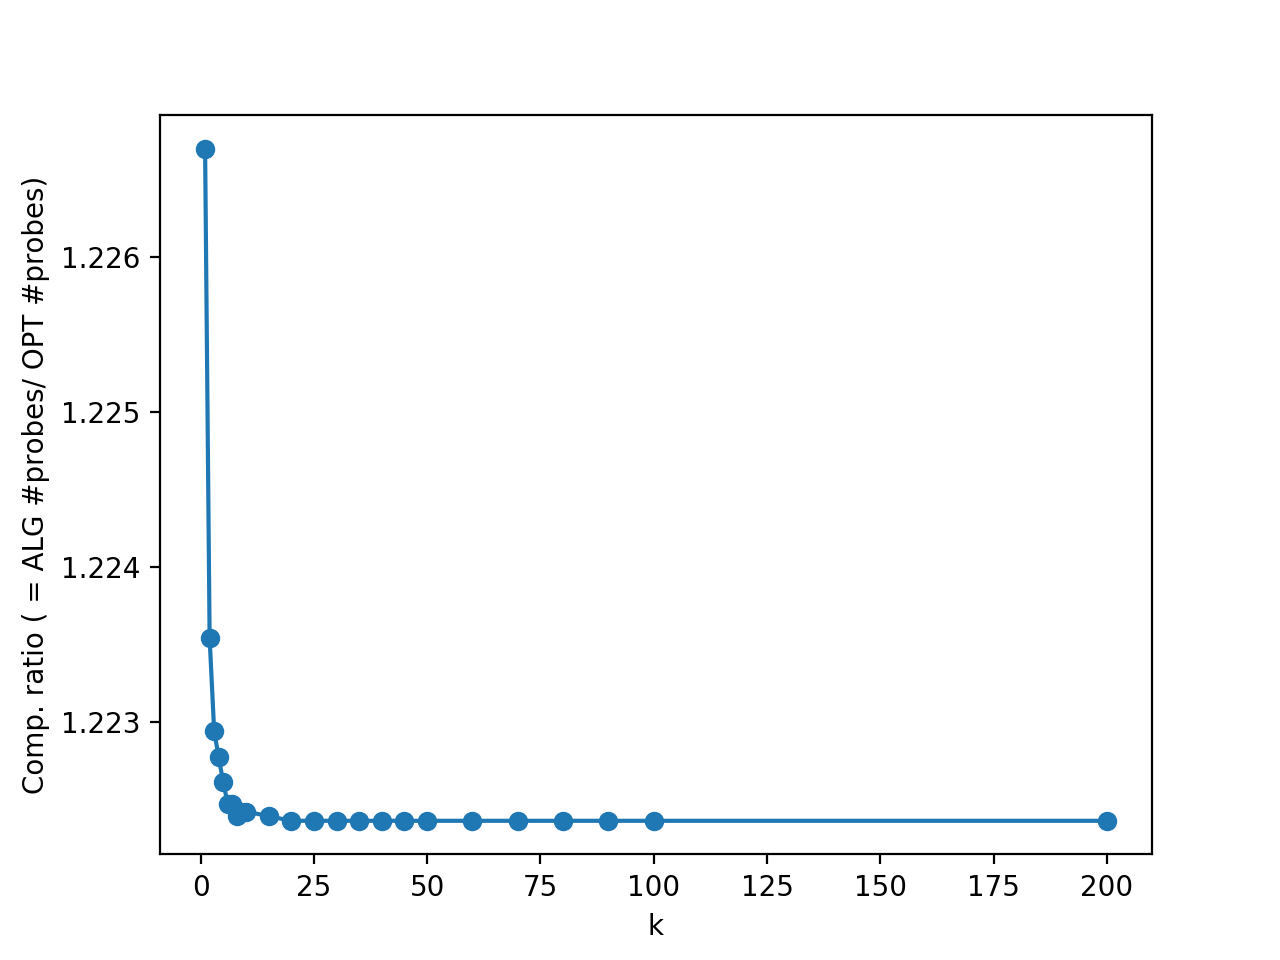
\includegraphics[height=0.7\textheight,keepaspectratio]{cr-k-uniform}
  \end{figure}
\end{frame}




\begin{frame}[noframenumbering]

  \frametitle{Competitive Ratio vs.\ $k$ on Adversarial Data}
  \begin{itemize}
      \item Adversarial data set constructed such that LIP-$k$ has worst case performance for odd $k$
      \item Run on query with $N = 2$ joins
  \end{itemize}
  \begin{figure}
    \centering
    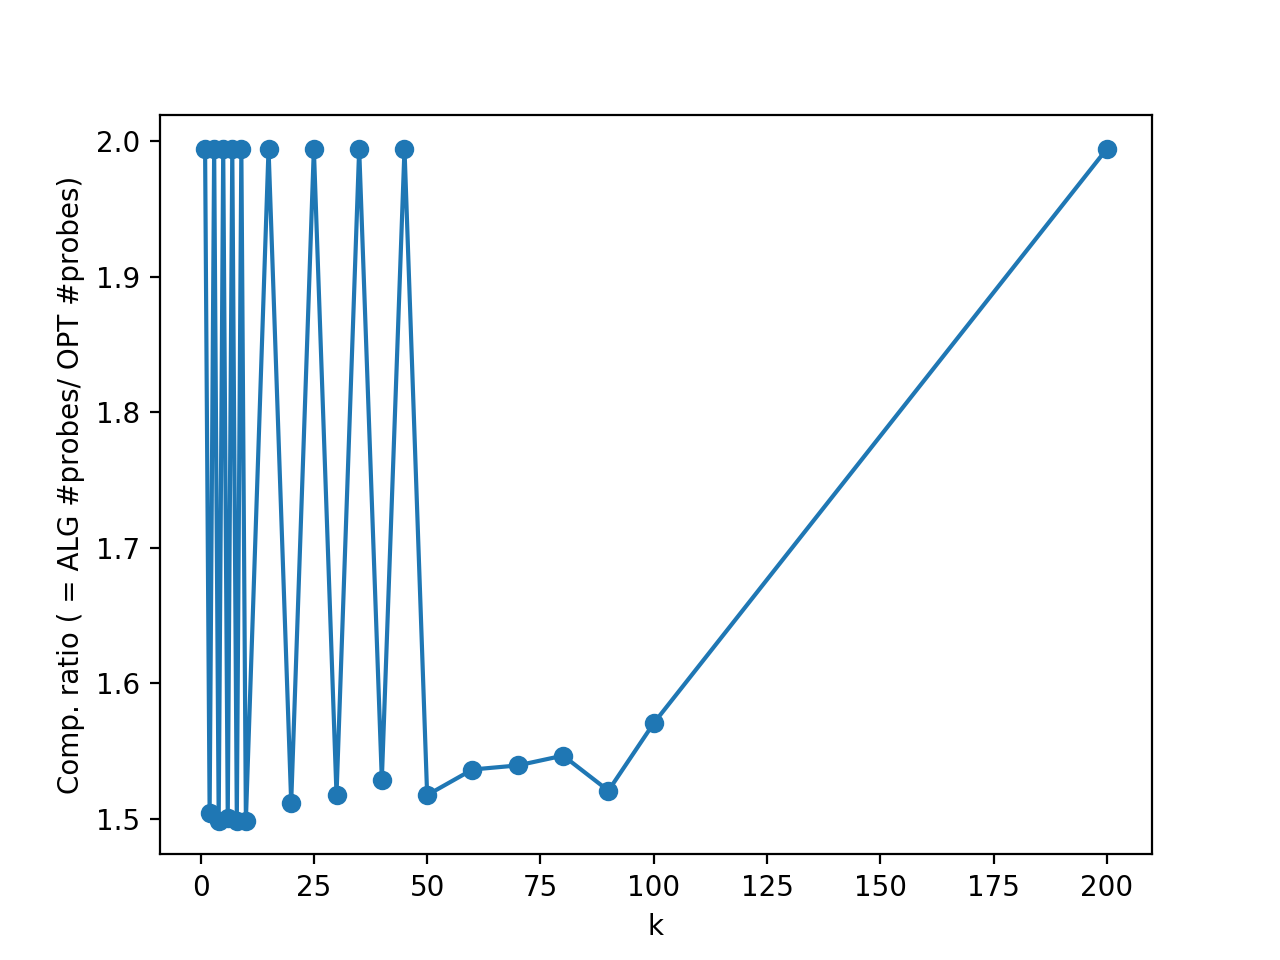
\includegraphics[height=0.7\textheight,keepaspectratio]{cr-k-skewed}
  \end{figure}
\end{frame}




\end{document}